\documentclass[runningheads]{llncs}

\usepackage[T1]{fontenc}

\usepackage{cite}
\usepackage{graphicx}
\usepackage{amsmath}
\usepackage{float}
\usepackage{enumitem}
\usepackage[linesnumbered,ruled,vlined]{algorithm2e}
\usepackage{todonotes}
\usepackage{wrapfig}
\usepackage[font=small,skip=4pt]{caption}
%\usepackage[disable]{todonotes}
\newcommand{\cmt}[1]{\todo[inline,color=green!40]{#1}}
%\newcommand{\assignment}[1]{}

\setlength{\intextsep}{6pt}
\setlength{\textfloatsep}{6pt}
\setlength{\floatsep}{6pt}
\captionsetup{skip=4pt, belowskip=0pt, aboveskip=4pt}

\setlistdepth{3}
\setlist[enumerate,1]{label=\textbf{\arabic*.}, ref=\arabic*}
\setlist[enumerate,2]{label=\textbf{\theenumi.\arabic*.}, ref=\theenumi.\arabic*}
\setlist[enumerate,3]{label=\textbf{\theenumii.\arabic*.}, ref=\theenumii.\arabic*}

\bibliographystyle{plain}
\begin{document}

\title{Natural Deduction Proofs for Educational Feedback}

\author{Daniel Macau\inst{1}
\and Ricardo Gonçalves\inst{1}
\and João Costa Seco\inst{1}}

\institute{NOVA School of Science and Technology, Caparica, Portugal}

\maketitle 

\begin{abstract}
Online tools, where students can practice and have automatic feedback, have shown to be useful both for MOOCS or as complementary material for traditional classes. Nevertheless, contrary to the myriad of tools that exist for learning programming languages, in the area of logic, a fundamental subject in any Computer Science programme, there is still a lack of such online tools, and in particular for the challenging exercise of Natural Deduction (ND) proofs. The few existing tools usually do not provide effective feedback, which is in fact challenging since tree-like ND proofs are non-linear and some steps are not immediate, as it is the case of proofs by contradiction. In this paper, we present an algorithm for pedagogical purposes that can generate human-readable ND proofs for a given problem. The algorithm supports both Propositional and First-Order Logic, and is based on hypergraphs. This allows obtaining the shortest and most direct proof for a given problem, but it can also adapt to a user’s current unfinished proof, allowing for greater flexibility in the proof construction. The algorithm can be integrated with educational platforms to guide users through the proofs by providing advanced feedback, at the same as it can help teachers grading ND exercises. 

\keywords{Natural Deduction  \and Propositional Logic \and First Order Logic \and Automation \and Algorithm \and Feedback \and Grading}
\end{abstract}


\section{Introduction}

Learning logic is fundamental in many fields, including programming, databases, AI, and algorithms~\cite{logicincomputer}. Among logic topics, ND stands out for its role in developing students’ reasoning skills~\cite{autogeneratingnd}, crucial for structured thinking and argumentation~\cite{vonPlato_2014}. ND exercises are challenging due to their complex reasoning and numerous rules, which students often find hard to apply correctly. Keeping track of multiple steps and assumptions can be confusing, leading to difficulties in mastering these exercises.
%Learning logic is a fundamental component of today’s curriculum, as it plays a key role in several important areas, including programming languages, databases, artificial intelligence, and algorithms~\cite{logicincomputer}. Logic courses cover a wide range of topics, and one that stands out is ND, given its importance in helping students develop reasoning skills~\cite{autogeneratingnd}, which are valuable in real-world contexts where structured thinking and argumentation are required~\cite{vonPlato_2014}.

%Natural deduction exercises are generally considered among the most challenging for students due to the complex reasoning involved. Since mastering them requires extensive exposure, many students struggle to become familiar with the rules and the formal way of thinking. These exercises involve numerous logical rules, and it is not always clear which one to apply. Additionally, students often need to keep track of multiple steps and assumptions simultaneously, which can be confusing.

Despite this importance, few online tools effectively support ND learning. Existing tools generally offer limited feedback, focusing on syntax or semantics but failing to guide students through conceptual challenges~\cite{Perh__2025}. Students often get stuck when unable to proceed or when overcomplicating solutions. This situation reveals the need for advanced feedback systems that generate complete proofs to guide students effectively. However, most existing algorithms lack flexibility, depend on specific ND systems, and cannot adapt dynamically to a user’s reasoning. Personalized feedback aligned with the student’s approach remains a challenge.
%Despite the importance of logic education, there remains a lack of online tools that support this type of exercise. The few existing tools typically offer very limited feedback, focusing mainly on syntactic and semantic errors while failing to provide deeper guidance that could help students overcome conceptual difficulties~\cite{Perh__2025}. A major challenge students face when solving ND problems is becoming stuck either because they reach an impasse or feel they are overcomplicating the exercise.

%This highlights the need for more advanced and effective feedback systems to address these gaps. One approach to producing this type of feedback is through algorithms capable of generating complete proofs. This allows the system to derive hints from the generated proof, ensuring that the guidance leads to a correct solution rather than a dead end. However, most existing algorithms were not developed for this purpose: while they can find a solution or detect contradictions, they often lack flexibility in terms of rule application, depend on the specific ND system used, and cannot dynamically adapt to a user’s reasoning process. Capturing the user’s reasoning enables the feedback to be personalized and aligned with the student’s chosen path.

In this article, we present an algorithm developed with a pedagogical focus to support building and verifying ND proofs. The algorithm generates multiple Gentzen-style proofs for problems in Propositional Logic (PL) and First-Order Logic (FOL). Using directed hypergraphs, it captures multiple valid proof paths and adapts to the user’s reasoning, providing step-by-step guidance. Using graph search methods, the system finds correct and shortest proofs, allowing it to give feedback on how good the solution is and track student progress.
%In this article, we present an algorithm developed during a thesis project with a pedagogical focus. It was originally created to support an application that helps students build and verify ND proofs. However, the application itself is not addressed in this article.  The algorithm is capable of automatically generating multiple Gentzen-style proofs for the same problem in a human-readable way, both in PL and FOL. A distinguishing feature of our algorithm is its ability to adapt to a user’s solution, providing step-by-step guidance that aligns with the student’s reasoning process. This is made possible through the use of directed hypergraphs that store information about which rules can be applied at each step, capturing multiple valid proof paths. By leveraging well-known graph search and traversal algorithms, the system not only finds correct solutions but also identifies the shortest proofs, enabling feedback on how a solution could be improved. Additionally, the algorithm can be used to assess exercises by determining how far a student’s resolution is from a valid or optimal solution, thereby offering a measurable assessment of proofs.
%!TEX root =  ../samplepaper.tex
\section{Background}
Proof systems are fundamental in logic education because they provide a structured framework for understanding and constructing logical arguments, ensuring rigor and validity in mathematical reasoning. Among the many proof systems, one usually adopted in the logic courses is the Natural Deduction (ND) system, which was defined to more closely align with mathematical and everyday reasoning under assumptions~\cite{nd-mancosu}. It emerged in 1934 with Gentzen and Jaśkowski's work, gaining widespread acceptance by the 1960s~\cite{Pelletier1999-FRAABH}. In a ND system we can construct proofs showing that a formula \(\varphi\) is a logical consequence of a set of formulas \(\Gamma\), written \(\Gamma \vdash \varphi\). 
%\cmt{O documento Gouveia e Dionisio nao deve ser citado por ser apenas um draft. Já agora, podemos usar este comando para deixar comentários ao longo do texto. Depois é fácil desativar todos de uma só vez.}
Even within ND, there are many ways to represent proofs. The two main styles are the Gentzen-style, which organizes the proof in a tree-shaped structure, also known as deduction tree, and the Fitch style, which uses a linear structure with deeper indentation levels to represent assumptions or intermediate steps in the proof. Our article focuses on the first one. 

Gentzen style trees represent proofs, and each node of the tree is a formula. The most basic tree is compose of just a formula, and more complex trees are obtained from these by successively applying inference rules. Rules are represented using horizontal lines, where its hypotheses appear above the line and the rule’s conclusion appears below. Since some of these inference rules have hypothetical assumptions, Gentzen-style ND uses natural number marks on the leafs of a tree as a mechanism to reference such hypothesis. An hypothesis (tree leaf) is considered discharged or closed if its mark is referenced by a rule applied below in the tree, meaning that this hypothesis is an assumption of such rule. If it is not close, an hypothesis is said to be open. The rule’s name and the corresponding marks for the hypotheses are placed on the right-hand side of the fraction representing the application of the rule.
Given a complex tree, the formula at its root is called the conclusion of the proof, and formulas at the leaves are called hypotheses.   

Regarding the inference rules, we will consider the usual classical logic rules. For each classical connective or quantifier $\Delta$, we have two rules: introduction rule ($\Delta_I$), which constructs more complex formulas from simpler ones, and elimination rules ($\Delta_E$), which extracts information from complex formulas. Additionally, a special rule, known as absurdity (\(\bot\)), allows deriving any conclusion from an explicit contradiction $\bot$. Some rules can only be applied under specific circumstances, called side conditions. For simplicity, we will not detail these here, but we take them into consideration in the algorithm. Figure \ref{fig:nd-rules} lists the complete set of classical rules we consider. Greek letters represent generic formulas, symbols of the form \( \mathcal{D} \) represent subtrees within branches, \( m \) and \( n \) denote marks, and \(\displaystyle \varphi^m\) over \( \mathcal{D} \) represents the fact that $\varphi$ can be used as an assumption in \( \mathcal{D} \).
%\cmt{RG: Acho que a notação está vaga porque usámos a mesma notação "[ ]" para coisas diferentes (o que nunca é boa ideia).}
With \(\displaystyle \left[ \varphi \right]^x_{\substack{t}}\) we represent the result of substituting free occurrences of $x$ with $t$ in $\varphi$.


\begin{figure}[h]
    \centering
    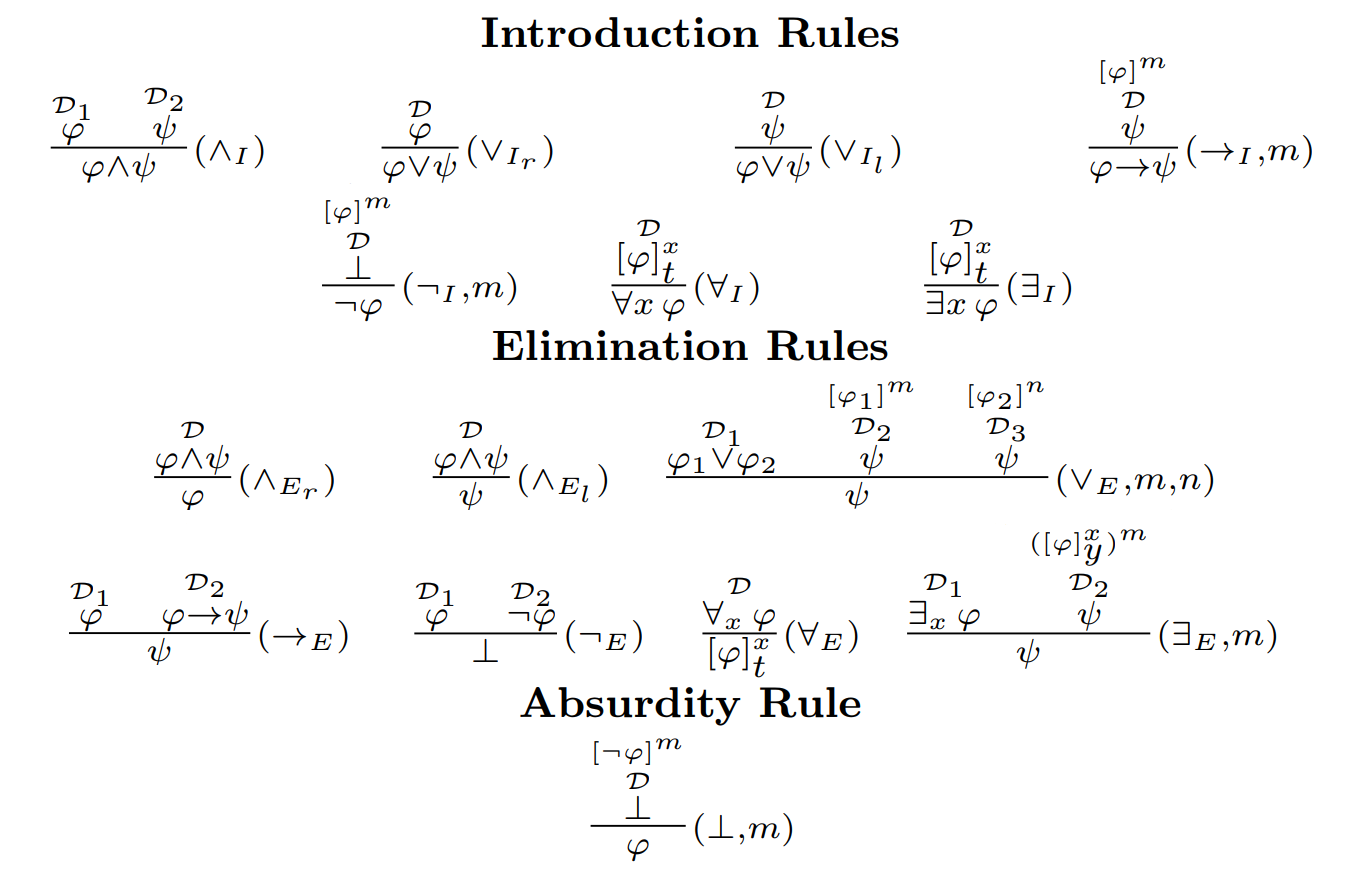
\includegraphics[width=1\linewidth]{resources/rules.png}
    \caption{List of rules for both PL and FOL}
    \label{fig:nd-rules}
\end{figure}

%These proofs can be constructed either bottom-up, from the conclusion to the hypotheses, or top-down, from the hypotheses to the conclusion.  --- talvez não valha a pena dizer isto aqui.

A ND proof is said to be well-formed if and only if it is finite and the inference rules are applied correctly. Moreover, we say that a ND proof proves the consequence \(\Gamma \vdash \phi\) if and only if it is well-formed, the root of the tree is \(\phi\), and every open hypothesis in the tree is contained in \(\Gamma\).
In Fig.~\ref{tab:proof-tree} we have an example of a well-formed ND proof of \( \{\neg (\varphi \lor \psi)\} \vdash \neg \psi \).

\begin{figure}[h]
    \centering
    \[
    \frac{\displaystyle \frac{
    \displaystyle \neg (\varphi \lor \psi)^1 \quad \displaystyle \frac{\psi^2}{(\varphi \lor \psi) \strut} \quad (\lor_{I_l}) \strut}
    {\displaystyle \bot \strut} \quad (\displaystyle \neg_E)\strut} {\displaystyle \neg \psi \strut} \quad (\neg_I, 2)
    \]
    \caption{ND tree proving \( \{\neg (\varphi \lor \psi)\} \vdash \neg \psi \).}
    \label{tab:proof-tree}
\end{figure}
%\begin{definition}[Well-Formed Tree Proof]
%A tree proof is well-formed if and only if it is finite and applies the inference rules correctly.
%\end{definition}
%
%\begin{definition}[Consequence Proven by a Proof]
%Given a tree proof and a problem \(\Gamma \vdash \phi\), we say that the tree solves the problem if and only if it is well-formed and the following conditions both hold:
%\begin{enumerate}
%    \item The root of the tree is \(\phi\).
%    \item Every open hypothesis in the tree is contained in \(\Gamma\).
%\end{enumerate}
%\end{definition}
%!TEX root =  ../samplepaper.tex
\section{Requirements}
Before we introduce the proposed algorithm, we must clarify its main goal. We want our algorithm to be able to support advanced feedback for students learning and practicing ND proofs. Such effective feedback system should be able to deliver relevant information to assist students at any stage of their exercise resolution. Focusing on this main goal, we identified four fundamental aspects a well-designed feedback system should satisfy:

\begin{itemize}

\item \textbf {Providing guidance on rule applications:} Some rule applications in ND are not obvious, making it difficult for students to progress. A paradigmatic example is the case of proofs by contradiction, which is a distinctive feature of classical logic. In some cases no direct proof exists, and the result can only be proved by contradiction: \(\varphi\) is proved by assuming \(\neg \varphi\) and showing that this leads to a contradiction. The feedback system should be able to identify such situations and suggest the appropriate rule applications.

\item \textbf {Breaking proofs into smaller sub-proofs:} Proofs in ND are incrementally built from smaller proofs. Dividing proofs into smaller steps reduces the cognitive load and simplifies reasoning. Therefore, the feedback system should encourage students to start with smaller proofs and incrementally build the main proof. 

\item \textbf{Indicating the distance to a solution:} Showing how many steps (rule applications) are needed to complete the proof helps students maintain focus and gain a clear sense of progress.

\item \textbf{Improvements in the proof:} Providing feedback about irrelevant steps taken or possible shortcuts that could make the proof clearer. It should also allow visualizing different ways to tackle the same problem.

\end{itemize}
Designing an algorithm that provides the basis for a feedback mechanism satisfying the above requirements is quite challenging. We aim to provide structured and clear information, as a tool for helping students to overcome the usual challenges of producing ND proofs.
%!TEX root =  ../samplepaper.tex
\section{Algorithm}
Our algorithm is structured in the three sequential steps discussed in this section.
We next present our algorithm that allows advanced feedback for ND exercises.

%The first step is to generate a hypergraph based on the main goal (what the exercise asks us to prove) and the target goal (the part of the student's proof we want to complete), in order to store all possible rule applications for both goals. Then, we use this graph to build a second hypergraph that simulates as many proof constructions as possible by decomposing the target goal into sub-goals. In the last step, we trim this second graph so that it retains only valid and minimal proofs, either in terms of the number of steps required or the height needed to solve the problem. Finally, we use the resulting graph to extract and build readable proofs, which can later be used to generate feedback.

\subsection{Transition Graph}
\cmt{RG: Estes dois parágrafos inicias precisavam de alguma revisão (em termos de apresentação das ideias), mas não consegui fazer. Posso voltar a isto depois.}
The first step is to create the so-called Transition Graph (TG). This graph stores the formulas that might be part of the final proof, as well as the rules that can be applied to each formula. 
To generate the graph, we need to specify what the consequence we want to prove \(\Gamma \vdash \varphi\), and the target goal \(\Sigma \vdash \theta\), which is the part of a student's proof that needs to be completed. The main goal is used to generate all the natural proof paths, which are proofs built using only formulas derived from decomposing the main goal. The target goal, on the other hand, can sometimes be used to generate non-natural proof paths. By this, we mean proofs that include more complex formulas than those directly derived from the main goal. By considering both goals, the system is able to generate more personalised and user-guided proofs, as it also takes into account the deviations made by the user, which is one of the core elements of our algorithm. For the type of information we want to store, we will make use of a special type of graph.

\begin{definition}[Labeled Directed Hypergraph with Labeled Heads]
A \emph{Labeled Directed Hypergraph with Labeled Heads} is a pair $H = (V, E)$, where:
\begin{itemize}
  \item \( V \) is a finite set of nodes, and
  \item \( E \subseteq V \times \mathcal{P}(V \times (V \cup \{\varepsilon\})) \times L \) is a finite set of labeled hyperedges, over a finite set of labels $L$, where each hyperedge $(t,\{(h_i,\ell_i): i\in I\}, \ell)$ consists of:
  \begin{itemize}
    \item a tail $t$, representing a single input node from \( V \),
    \item a set of labeled heads, which is a set of pairs \( (h_i, \ell_i) \in V \times (V \cup \{\varepsilon\}) \), where \( h_i \) indicates one of the output nodes and \( \ell_i \) is its label, which is either a node or the empty symbol \( \varepsilon \), and
    \item the global label $\ell$ of the hyperedge, which is an element of \( L \).
  \end{itemize}
\end{itemize}
\end{definition}

The Transition Graph (TG) we will construct is a hypergraph as defined above, where vertices are formulas and each hyperedge represents the application of an inference rule, which, as we have seen, may have mode than one premise. 
%
%
%\begin{definition}[Transition Graph]
%A \emph{Transition Graph (TG)} is a pair
%\[
%T_G = (F, T_E),
%\]
%where:
%\begin{itemize}
%  \item \( F \) is a finite set of \emph{formulas}, and
%  \item \( T_E \subseteq F \times \mathcal{P}(F \times (F \cup \{\varepsilon\})) \times R \) is a finite set of \emph{labeled hyperedges} called \emph{Transition Edge (TE)}, where each edge consists of:
%  \begin{itemize}
%    \item a tail formula \( f \in F \),
%    \item a set of pairs \( (f_1, f_2) \in F \times (F \cup \{\varepsilon\}) \), where \( f_1 \) is a \emph{hypothesis} and \( f_2 \) is a \emph{closed hypothesis}, and
%    \item a rule \( r \in R \).
%  \end{itemize}
%\end{itemize}
%\end{definition}
%
To give some intuition on the formal construction of TG, in \autoref{fig:te-ex} we can see  how the applications of rule \(\vee_E\) can be represented using hypergraphs.



    \begin{figure}[h]
        \centering
        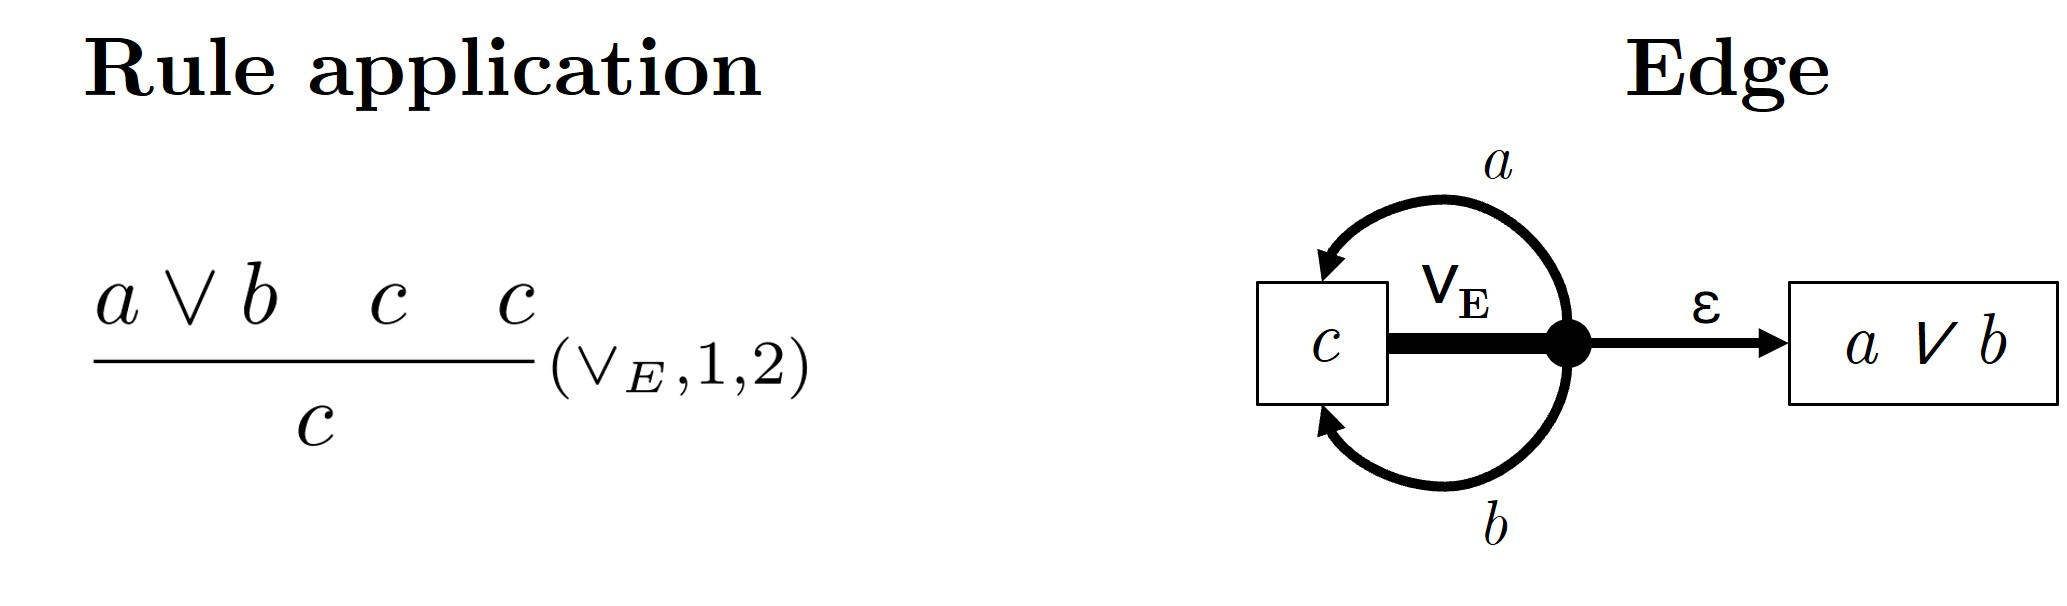
\includegraphics[width=0.8\linewidth]{resources/te-example.jpg}
        \caption{Example of a transition edge.}
        \label{fig:te-ex}
    \end{figure}

Formally, the above hyperedge is represented as $(c, \{(a \vee b, \varepsilon), (c, a), (c, b)\}, \vee_E)$. Edges go from the unique conclusion of the rule to its hypotheses. The labels of the heads of the hyperedge represent the possible additional hypothesis that can be used in that branch. In the above rule $\vee_E$, each side of the disjunction can be used as an additional hypothesis in the second and third branches of the rule, encoding the reasoning by cases. 
If we were working with FOL proofs, we would also need to consider side conditions as part of TG. 
%The reason for using this type of graph is that it allows us to map rule applications directly into a data structure. 
%In the final step, we will explain why it is necessary to store edges in this way. 
%Also, at this point of the construction, there is no need to keep track of the marks. We will see later that we can easily deal with these in the final step of the construction.

%\vspace{1em}
We present, in \autoref{alg:tg-construction}, the concrete procedure to generate the TG.
\begin{algorithm}[h]
\caption{Transition Graph Construction}
\label{alg:tg-construction}
\KwIn{Main goal $\Gamma \vdash \varphi$, Target goal $\Sigma \vdash \theta$}
\KwOut{Transition Graph $T_G = (F, T_E)$}

$F \leftarrow \Gamma \cup \Sigma \cup \{\varphi, \theta\}$ \tcp*[r]{Initialize formulas}
$T_E \leftarrow \emptyset$ \tcp*[r]{Initialize edges}

\tcp{Compute formulas}
\ForEach{$f \in F$}{
  \If{$f $was not already added as a negation}{
    $F \leftarrow F \cup \{\lnot f\}$ \tcp*[r]{Add negation for indirect rules}
  }

  Decompose $f$ into parts $S$\;
  $F \leftarrow F \cup S$\;
}

\tcp{Compute transitions}
\ForEach{$f \in F$}{
    
    \If{$f$ was not added as a negation}{
        $T_E = T_E \cup \{(f, \{(\bot, \lnot f)\}, \bot)\}$\;
    }

    \If{$f = \lnot \alpha$ for some $\alpha$}{
        $T_E = T_E \cup \{(\lnot \alpha, \{(\bot, \alpha)\}, \lnot_I)\}$\;
        $T_E = T_E \cup \{(\bot, \{(\alpha, \varepsilon), (\lnot \alpha,\varepsilon)\}, \lnot_E)\}$\;
    }

    \If{$f = \alpha \lor \beta$ for some $\alpha, \beta$}{
        $T_E = T_E \cup \{(f, \{(\alpha, \varepsilon)\}, \vee_{I_R})\}$\;
        $T_E = T_E \cup \{(f, \{(\beta, \varepsilon)\}, \vee_{I_L})\}$\;
        \ForEach{$f' \in F$}{
            $T_E = T_E \cup \{(f', \{(f, \varepsilon), (f',\alpha), (f', \beta)\}), \vee_E\}$\;
        }
    }

    \If{$f = \alpha \land \beta$ for some $\alpha, \beta$}{
        $T_E = T_E \cup \{(\alpha \land \beta, \{(\alpha, \varepsilon), (\lnot \beta,\varepsilon)\}, \land_{I})\}$\;
        $T_E = T_E \cup \{(\alpha, \{(\alpha \land \beta, \varepsilon)\}, \land_{E_R})\}$\;
        $T_E = T_E \cup \{(\beta, \{(\alpha \land \beta, \varepsilon)\}, \land_{E_L})\}$\;
    }

    \If{$f = \alpha \to \beta$ for some $\alpha, \beta$}{
        $T_E = T_E \cup \{(\alpha \to \beta, \{(\beta, \alpha)\}, \to_{I})\}$\;
        $T_E = T_E \cup \{(\beta, \{(\alpha, \varepsilon), (\alpha \to \beta, \varepsilon)\}, \to_{E})\}$\;
    }

}

\end{algorithm}
As we said, we have as input the consequence we aim to prove \(\Gamma \vdash \varphi\) and a consequence \(\Sigma \vdash \theta\) representing a partial proof of an user. The computation of the relevant formulas and transitions between these can be done in just one loop, but, for the sake of simplicity of presentation, we kept these separated. For the formulas we just consider the set of all subformulas of the formulas contained in the consequence we want to prove and in the partial consequence, together with the negation of these formulas. This way, all formulas that could appear in ND proof of the main consequence are vertices of TG.
The hyperedges of TG correspond to the possible rule applications between these considered formulas.

%The decomposition step is an important part to know in advance which formulas we will have in the graph and also to match with formulas that require that information, since they can be applied to every formula, such as the Elimination of Disjunction rule. The decomposition is done by splitting the formula at the outermost logical operators (if it is not an atomic formula). For example, $a \to \lnot b$ can be split into $a$ and $\lnot b$, but $a$ cannot be decomposed since it is atomic. However, we can decompose $\lnot b$ into just $b$.

To illustrate the construction process, we present a full example in \autoref{fig:tg-final}. The main consequence and the partial consequence are both \(\vdash a \to a\).
\cmt{RG: Não percebo qual é o input neste caso: qual a main consequence e a partial consequence?}
\cmt{DM: Neste caso são o mesmo, por outras palavras, estamos a computar uma solução completa para o problema e não necessariamente a gerar feedback para um passo incompleto de uma prova, por isso main e partial = \(\vdash a \to a\). A minha ideia era ter feito um exemplo em que, de facto, se completasse uma prova mas o numero de nos e arestas cresce demasiado e nao consigo representar o grafo mesmo sendo um pequeno desvio ex: \(\{\lnot (a \to a)\} \vdash a \to \bot\) já ficamos com 6 nos e 12 edges}
\begin{figure}[h]
    \centering
    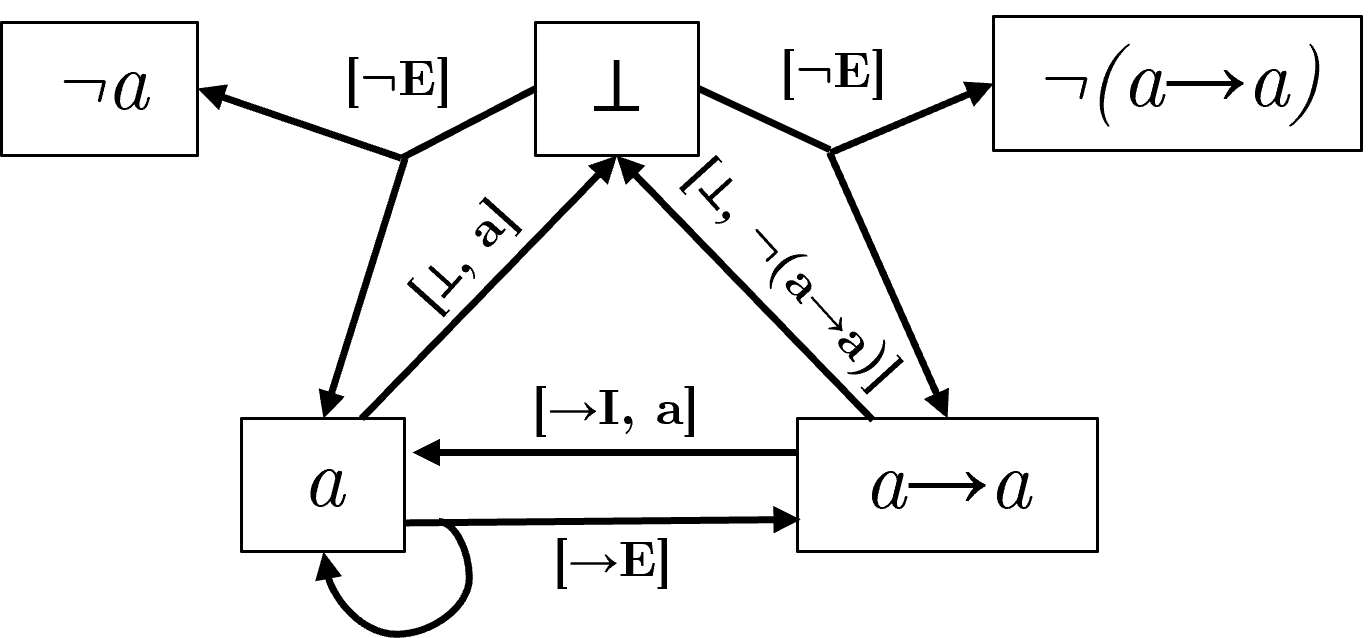
\includegraphics[width=0.8\linewidth]{resources/tg-final.png}
    \caption{Final TG generated from main goal and target goal \(\vdash a \to a\)}
    \label{fig:tg-final}
\end{figure}

\subsection{Proof Graph}
The second step is to build the Proof Graph (PG). The structure of this graph is very similar to the TG, but it stores different objects. It stores the possible sub-goals derived from the target goal. In this graph, the nodes are goals, and the edges are adaptations of transition edges (TE) that now store goals. The purpose of this graph is to decompose the target goal into smaller goals that are easier to prove, until we reach goals that can be directly proved. In the end, after generating all sub-goals, the graph may contain multiple proof paths. Some of these paths may not lead to a solution, while others may succeed in proving the target goal. In short, the PG aims to find the maximum number of different "game" combinations. To generate the PG, we use the TG, previously generated, and the target goal. Note that the target goal can also be the initial goal, in case we want to generate a full proof for the problem. Before we describe the procedure, we define some key terms:

\begin{definition}[Proof Graph]
A \emph{Proof Graph (PG)} is a pair $P_G = (G, P_E)$:
\begin{itemize}
  \item \( G \) is a finite set of \emph{goals}, and
  \item \( P_E \subseteq G \times \mathcal{P}(G \times (F \cup \{\varepsilon\})) \times R \) is a finite set of \emph{labeled hyperedges} called \emph{Proof Edge (PE)}, where each edge consists of:
  \begin{itemize}
    \item a tail goal \( g \in G \),
    \item a set of pairs \( (g_1, f_1) \in G \times (F \cup \{\varepsilon\}) \), where \( g_1 \) is a goal and \( f_1 \) is a \emph{closed hypothesis}, and
    \item a rule \( r \in R \).
  \end{itemize}
\end{itemize}
\end{definition}

\begin{definition}[Proved Goal]
A goal \( \Delta \vdash \delta \) is \emph{proved} if either:
\begin{itemize}
  \item \( \delta \in \Delta \), or
  \item there exists a Proof Edge \( (g, T, r) \in P_E \) in the Proof Graph \( P_G = (G, P_E) \), such that \( g = \Delta \vdash \delta \), and for every pair \( (g_1, f_1) \in T \), the goal \( g_1 \) is proved.
\end{itemize}
\end{definition}

The definition of proved goal is extremely important because it is used as a stopping condition to avoid the algorithm looping through unnecessary goals and to guarantee that the proof is valid. This is only possible due to the type of graph chosen, as it allows us to capture the relation between the hypotheses and the conclusion of each rule application. \autoref{fig:pe-ex} shows an example of a PE and how these relations can be captured. In the figure, we want to prove \(\{a \vee b\} \vdash a\). By applying the Elimination of Disjunction rule, we notice that one of the hypotheses cannot be closed using only this rule, even if the other two hypotheses are closed. So, what we actually prove with this rule is \(\{a \vee b, a\} \vdash a\), which is different from our goal. To accurately track which goals are proved and ensure the proof only contains valid proved goals, this information must be stored in a hypergraph structure. This is why hypergraphs are necessary.

\begin{figure}[h]
    \centering
    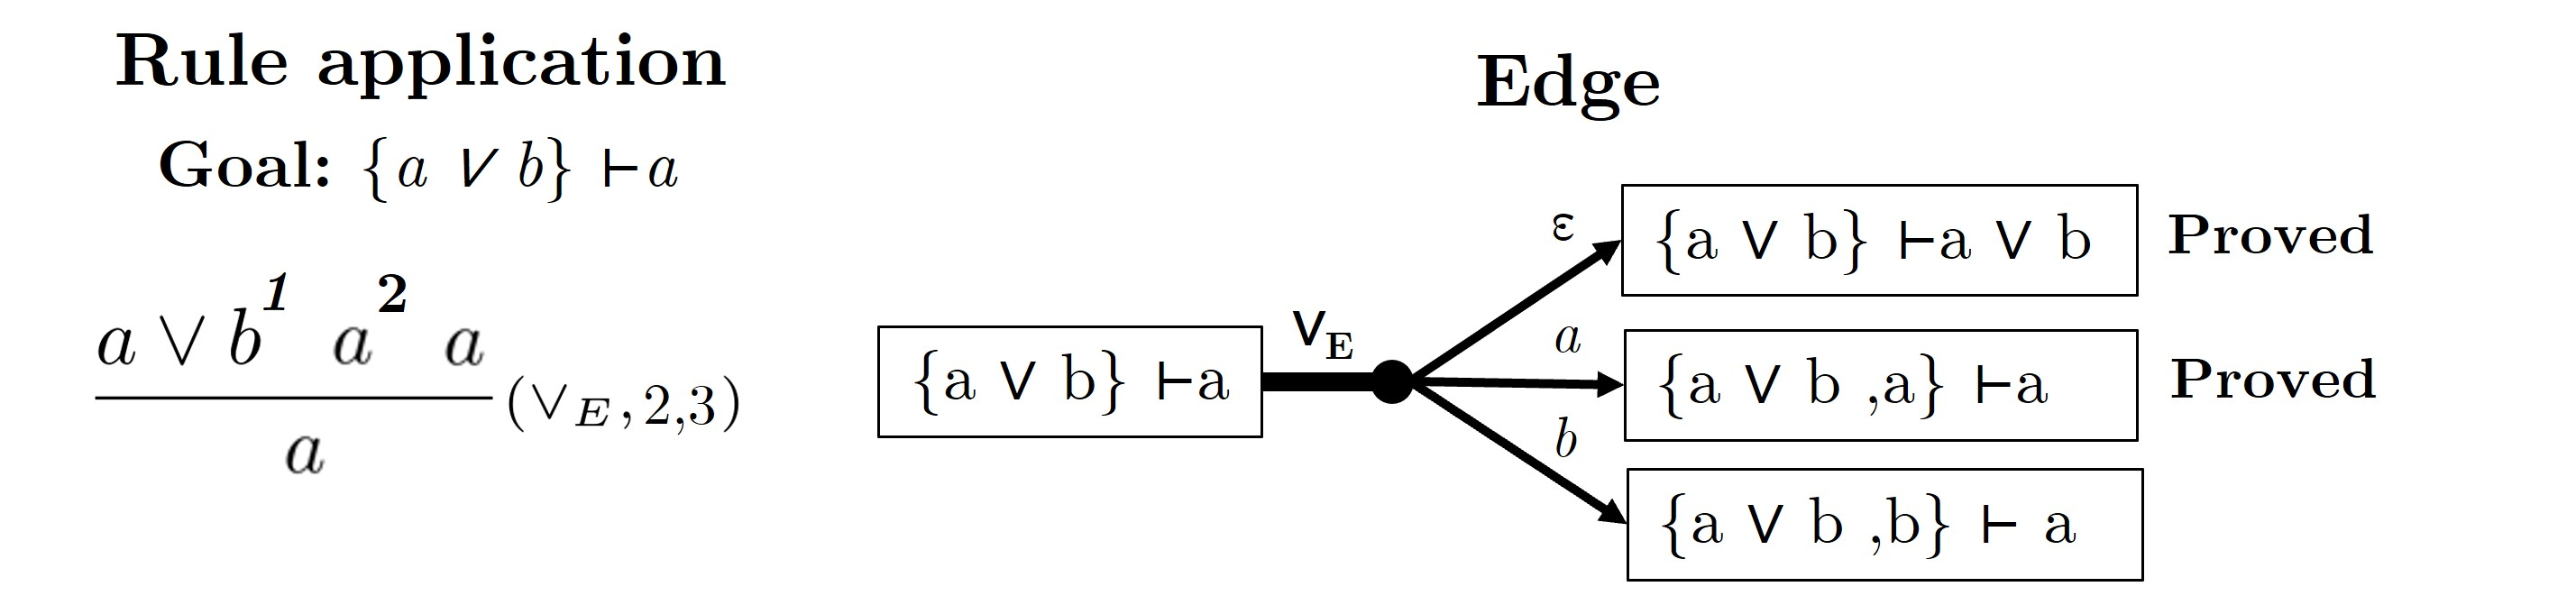
\includegraphics[width=1\linewidth]{resources/pe-example.jpg}
    \caption{Prove \(\{a \vee b\} \vdash a\) using the Elimination of Disjunction rule}
    \label{fig:pe-ex}
\end{figure}

\vspace{1em}
With all the necessary definitions in place, we now present the procedure to generate the PG, as shown in \autoref{alg:pg-construction}.

\begin{algorithm}
\caption{Proof Graph Construction}
\label{alg:pg-construction}
\KwIn{Transition Graph $T_G = (F, T_E)$, Target goal $t_g$}
\KwOut{Proof Graph $P_G = (G, P_E)$}

$G \leftarrow \{t_g\}$ \tcp*[r]{Initialize set of goals}
$P_E \leftarrow \emptyset$ \tcp*[r]{Initialize set of proof edges}

\tcp{Compute sub-goals}
\ForEach{$g = \Sigma \vdash \theta \in G$}{

    \If{$g$ is proved}{
        \textbf{continue} \tcp*[r]{Skip proved goal}
    }

    \If{stopping condition is reached}{
        \textbf{break} \tcp*[r]{Avoid excessive expansion}
    }

    \tcp{Get transition edges for formula $\theta$}
    $TE_\theta \leftarrow \{ (f, H, r) \in T_E \mid f = \theta \}$\;

    \ForEach{$(f, H, r) \in TE_\theta$}{
        $T \leftarrow \emptyset$  \tcp*[r]{Store transitions to each hypothesis}
        
        \ForEach{$(f_1, f_2) \in H$}{
            \tcp{Create sub-goal by extending the current premises with the closed hypothesis}
            $g_\text{new} \leftarrow (\Sigma \cup \{f_2\}) \vdash f_1$\;

            $T \leftarrow T \cup \{(g_\text{new}, f_2)\}$\;
            $G \leftarrow G \cup \{g_\text{new}\}$ \tcp*[r]{Add sub-goal}
        }

        $P_E \leftarrow P_E \cup \{(g, T, r)\}$ \tcp*[r]{Add proof edge}
    }
}
\end{algorithm}

This part of the algorithm can generate very large graphs, with millions of distinct goals depending on the complexity of the problem. In most cases, we do not want to explore the entire goal space, as many goals are extremely complex and do not provide useful feedback. Therefore, stopping conditions are required. These may include: limiting the total number of goals explored, setting a maximum number of hypotheses allowed per goal, or enforcing a timeout.

\autoref{fig:st-ex} shows the PG generated using the TG from \autoref{fig:tg-final} and target goal \(\vdash a \to a\), with a limit of 9 goals explored. Nodes with solid borders represent proved goals, while nodes with dashed borders represent unproved goals. Since our target goal is proved, we know that at least one solution was found.

\begin{figure}[h]
    \centering
    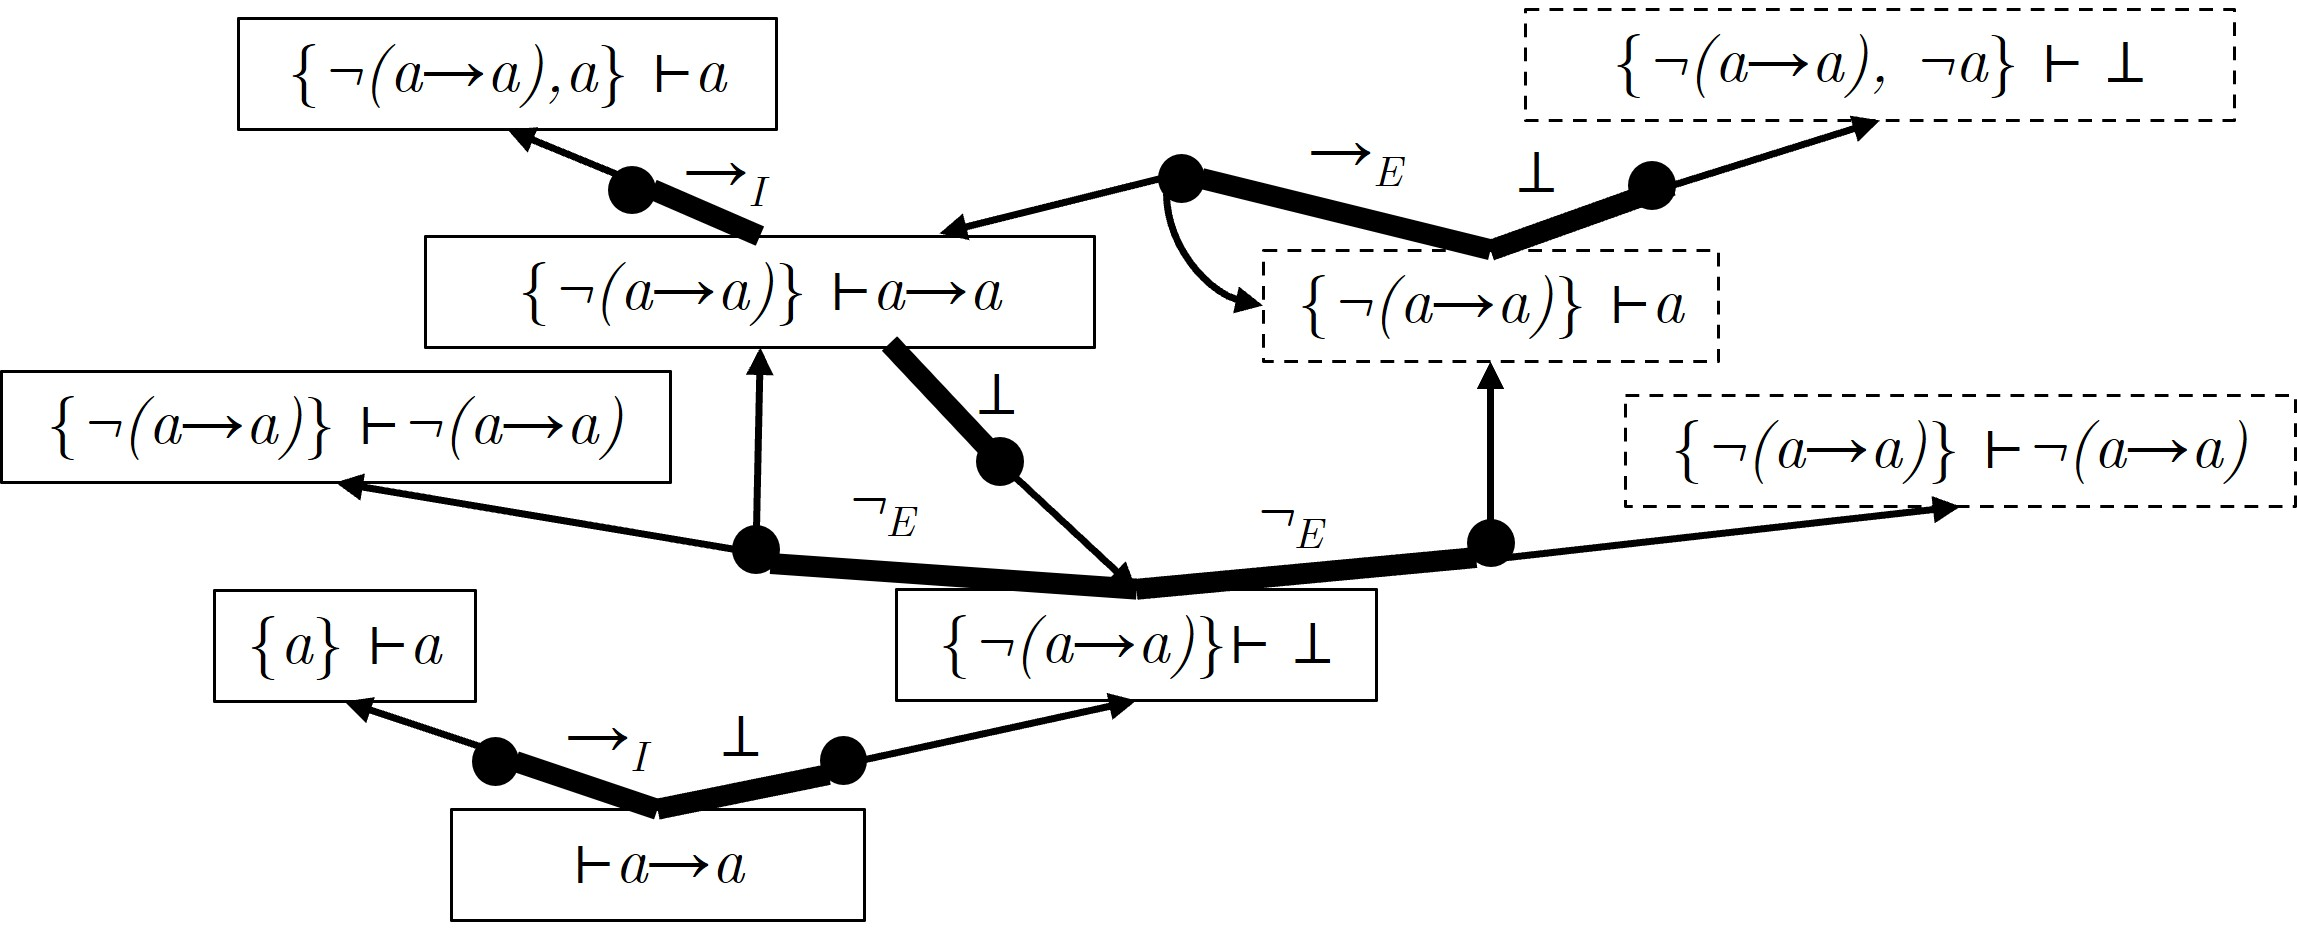
\includegraphics[width=0.8\linewidth]{resources/sg-gen.jpg}
    \caption{Example of Proof Graph using the TG from \autoref{fig:tg-final} and target goal \(\vdash a \to a\)}
    \label{fig:st-ex}
\end{figure}

\subsection{Proof Graph Trimming}

The final stage of our algorithm consists of trimming the PG to keep only the valid solutions of the problem. The resulting trimmed graph includes only proved goals and the edges that lead to the shortest proofs, where short proofs can be defined in two different ways: one based on height (Height Trim Strategy), and the other based on the number of formulas involved (Size Trim Strategy). Both strategies rely on a standard graph traversal technique, namely \emph{breadth-first search}, to determine which goals and edges should be preserved. The trimming process begins by iterating through all goals and discarding those that cannot be proved. Then, one of the following trimming strategies is applied:
\vspace{1em}

\textbf{Height Trim Strategy (HTS):} This algorithm traverses the PG in reverse order: it starts from the leaves and visits nodes using breadth-first search. Since this traversal guarantees that each node is first reached through the shortest possible path in terms of height, the algorithm retains only the first PE that reaches each goal. All other incoming edges to the same goal are discarded, even if other solutions exist with the same height.

\begin{figure}[h]
    \centering
    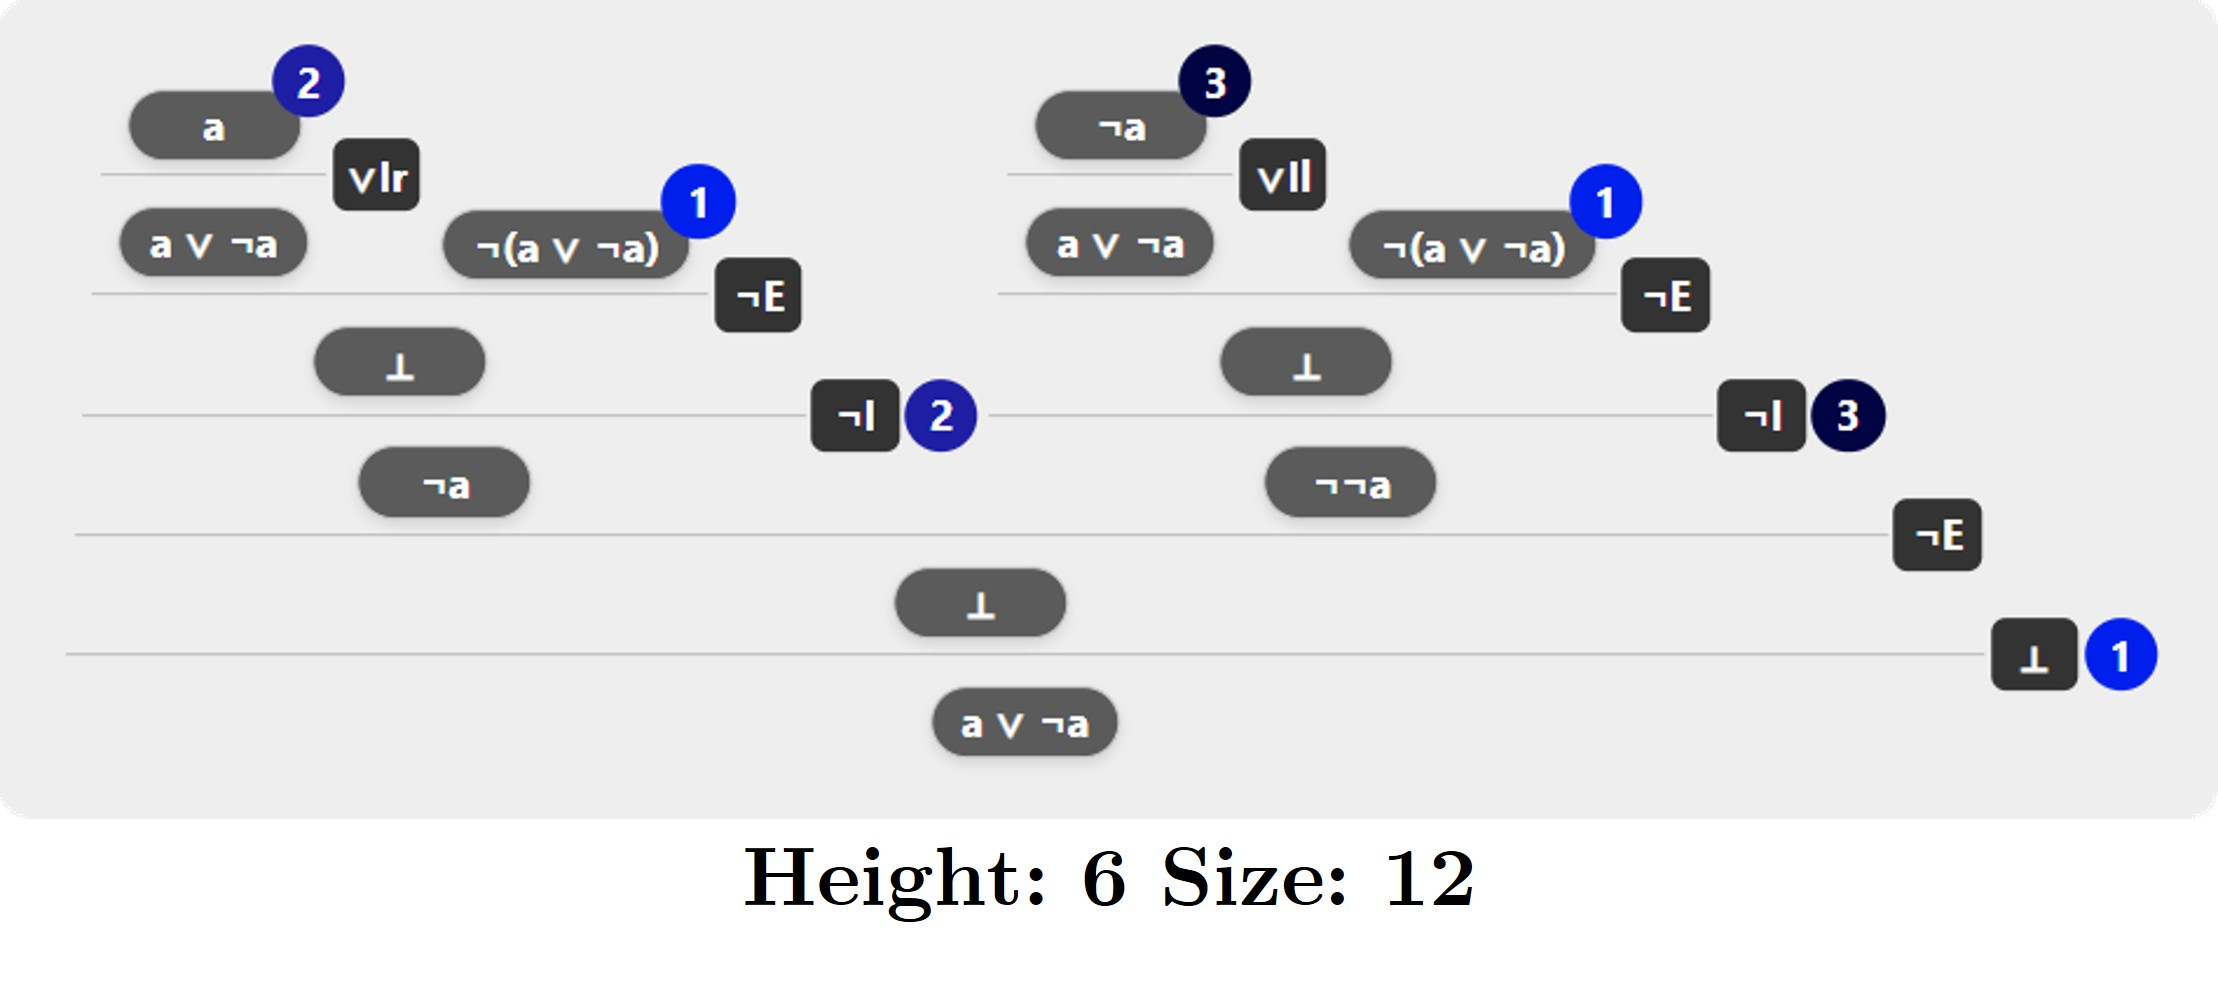
\includegraphics[width=0.6\linewidth]{resources/trim-height.jpg}
    \caption{Example of a full proof generated by the algorithm for \(\vdash a \vee \lnot a\), using HTS.}
    \label{fig:sg-trim-height}
\end{figure}

\textbf{Size Trim Strategy (STS):} This strategy is similar to HTS, but it tracks the size of each proof, defined as the number of formulas involved. Instead of retaining the first edge to reach a goal, it must explore all incoming edges to identify the one that yields the smallest proof. Consequently, a goal may be visited multiple times, making this strategy more computationally expensive. However, it often results in more concise proofs in terms of rule applications.

\begin{figure}[h]
    \centering
    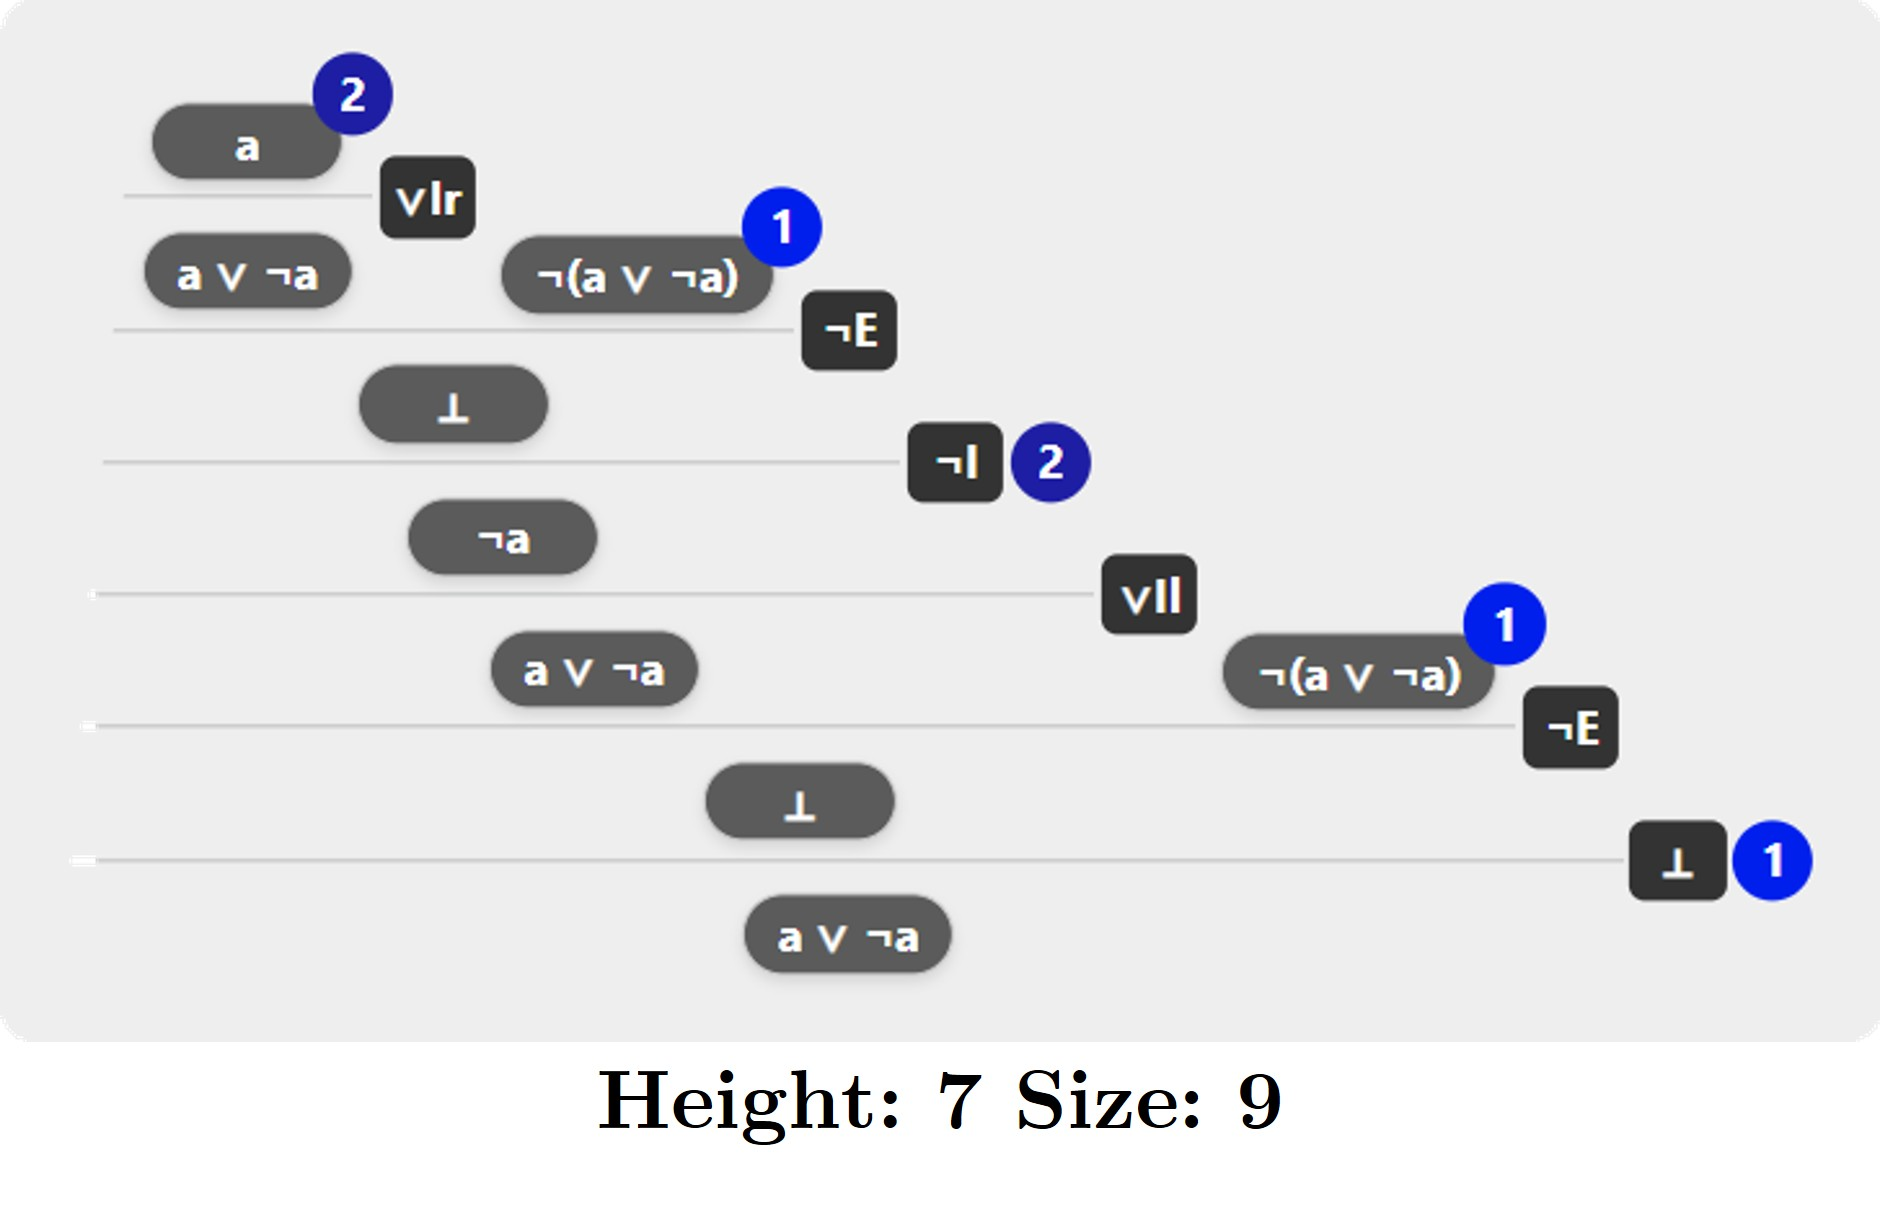
\includegraphics[width=0.6\linewidth]{resources/trim-size.jpg}
    \caption{Example of a full proof generated by the algorithm for \(\vdash a \vee \lnot a\), using STS.}
    \label{fig:sg-trim-size}
\end{figure}

Another key feature that distinguishes us from other algorithms is that we do not store just a single solution, but rather a set of possible solutions. This is important to avoid recomputing the entire algorithm when generating feedback for the same problem. However, it comes at a cost in terms of space, as it stores thousands of goals. The algorithm can be queried to generate a new feedback step if all formulas in the new target goal are contained in the set of formulas in the TG used to generate the final trimmed PG. \autoref{fig:sg-trim} shows the TG from \autoref{fig:st-ex} after being trimmed using STS. The algorithm found a solution \textbf{A} for the target problem and also solutions for each of the subgoals presented in the graph.
\begin{figure}[h]
    \centering
    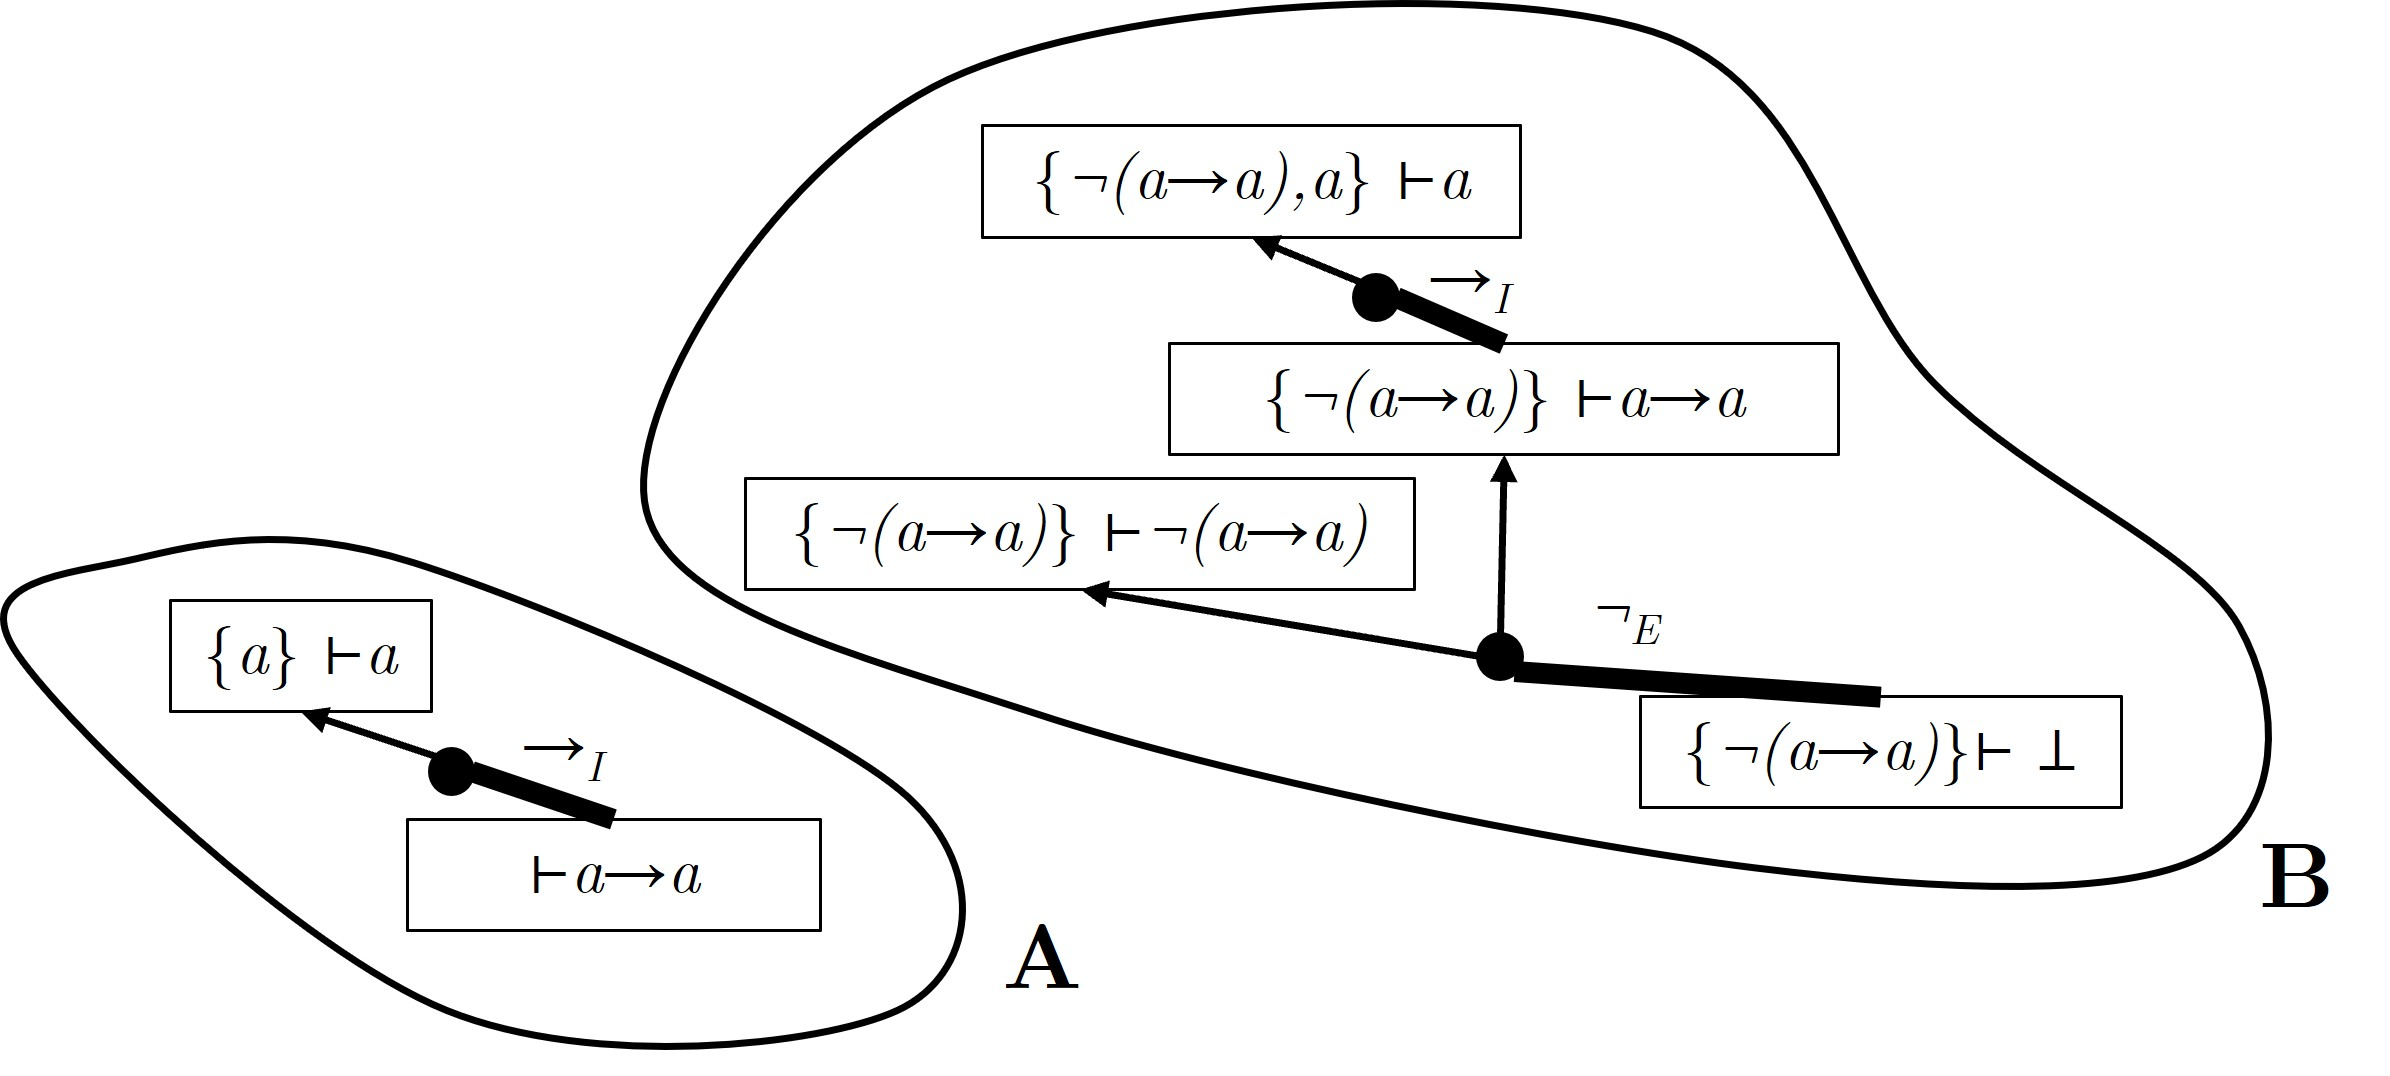
\includegraphics[width=0.8\linewidth]{resources/sg-final.jpg}
    \caption{Trimmed TG using STS.}
    \label{fig:sg-trim}
\end{figure}
\subsection{Feedback Generation}
With the final graph, we can now generate feedback by querying which goals remain unproved in the student's proof. \autoref{fig:extract-solution} and \autoref{fig:extract-solution2} illustrate examples of how feedback can be generated from the final graph.

In this first example, the student does not know how to proceed after applying the Absurdity rule. By querying the  graph with the goal that is still unproved, we get the solution \textbf{B} in \autoref{fig:sg-trim}. Knowing the remaining part of the proof, we can generate feedback. For example, we can tell the student to apply the Elimination of the Negation rule using \(a \to a \) and  \(\lnot(a \to a) \) (\textbf{Providing guidance on rule applications}). In this specific case, we cannot give hints about sub-proofs to solve the problem, as the solution is already small. But in some cases where the solution is bigger, we can do that (\textbf{Breaking proofs into smaller sub-proofs}). We can also specify how far the student is from the final proof. In this case, we can say that they are two rules away from completing the proof (\textbf{Indicating the distance to a solution}). Finally, we can also suggest some improvements in the resolution. In this case, the student shifts their solution by applying the Absurdity rule, making it longer. That information can also be extracted from the graph (\textbf{Improvements in the proof}).

\begin{figure}
    \centering
    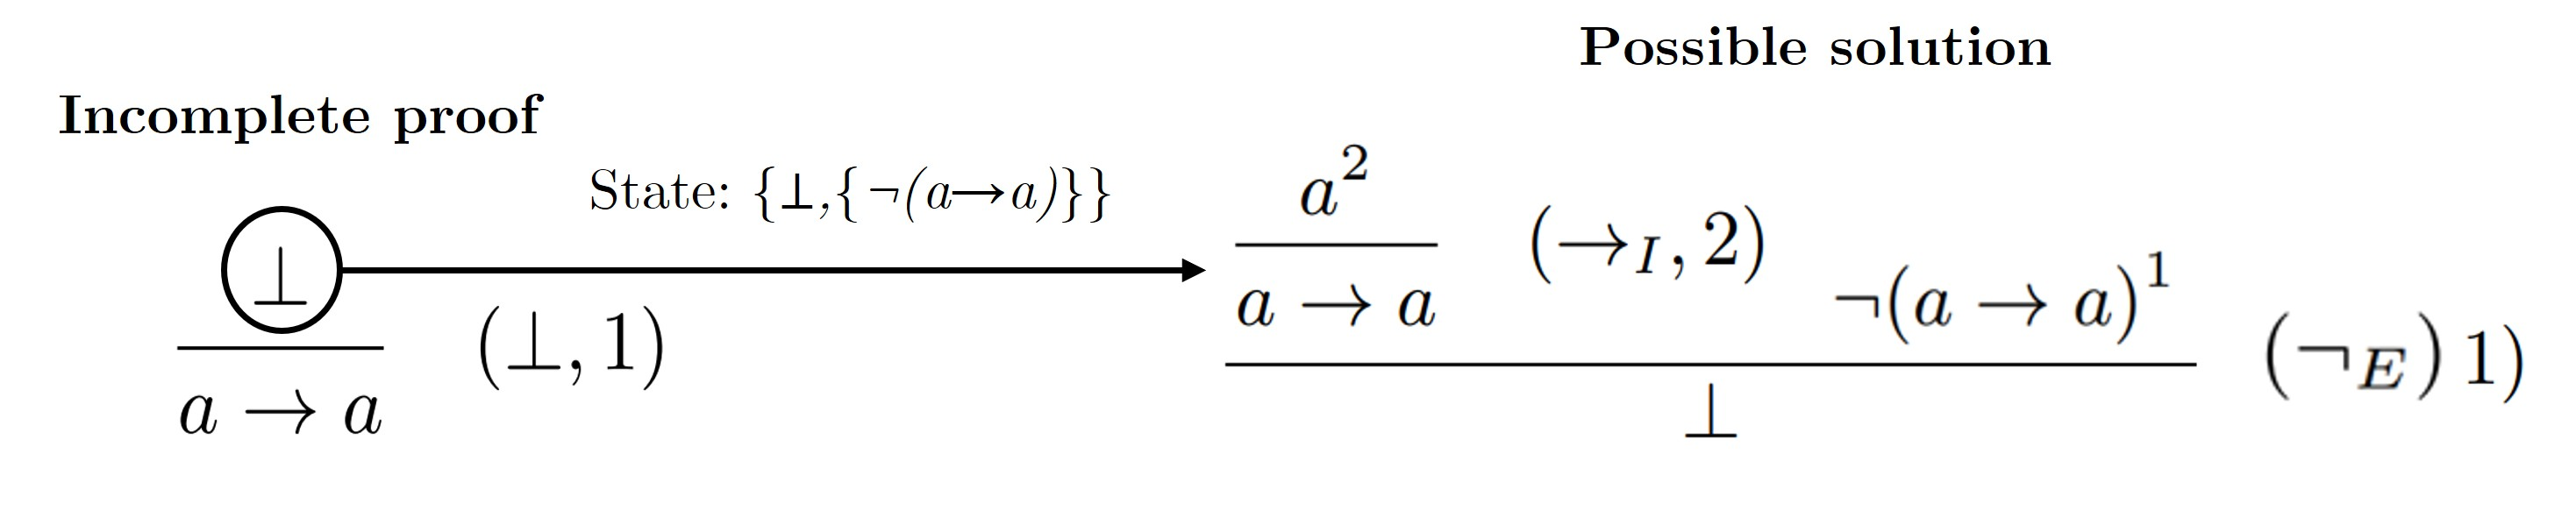
\includegraphics[width=1\linewidth]{resources/trim-pos-feed.jpg}
    \caption{Extracting a solution to produce feedback from a proved goal}
    \label{fig:extract-solution}
\end{figure}

In this second example, a solution cannot be found, as the goal assigned to the unresolved part of the proof does not belong to the final graph. In this case, we can inform the student that the path they are taking may be too complex, and we can suggest going back \(X\) rule applications until the algorithm finds the correct path again to guide the student. We cannot affirm that there is no solution, because we may not have explored the whole space of possible solutions. For example, the final graph was only constructed considering the first 9 nodes. In this example, if the student removes the Elimination of Negation rule (one step back), we return to the situation previously presented.
\begin{figure}[h]
    \centering
    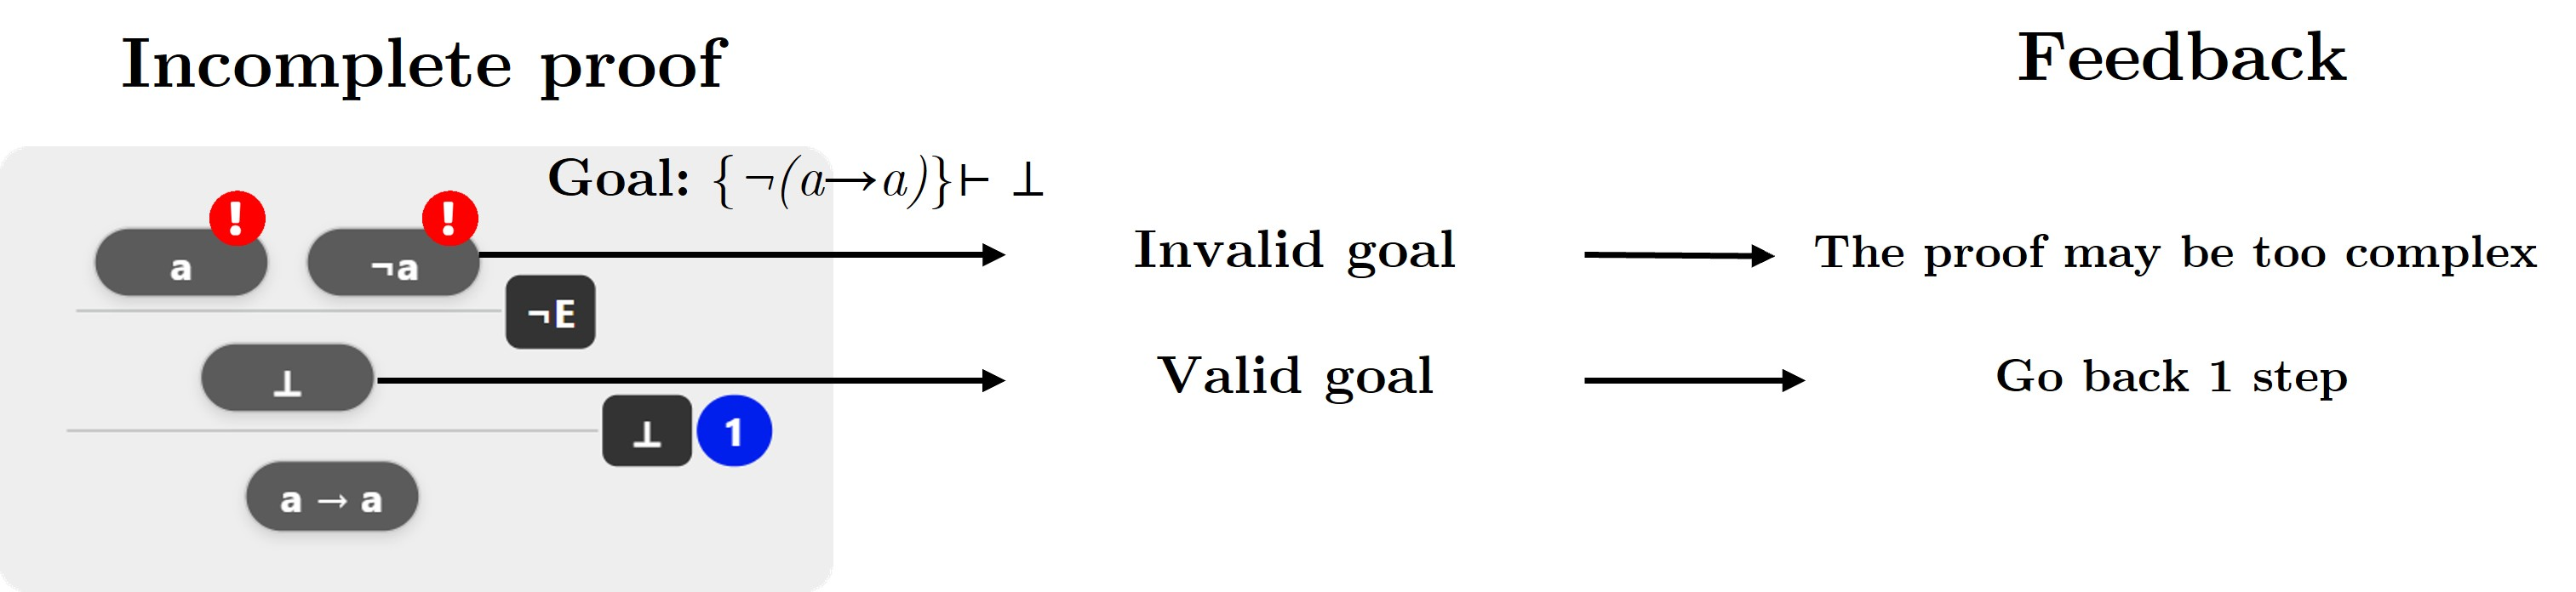
\includegraphics[width=1\linewidth]{resources/trim-neg-feed.jpg}
    \caption{Extracting a solution to produce feedback from an unproved goal.}
    \label{fig:extract-solution2}
\end{figure}
These methodologies can also be used to assess exercises. For example, we could compute how far a student’s resolution is from a possible solution, or how far it is from the best solution. In some cases, based on the size of the explored solution space, we can say that the student overcomplicated the resolution.

Our algorithm is already implemented and has been tested. It is already integrated in a visual online tool focused on ND proofs. Some of the figures shown are from this tool, which allows students to practice ND proofs.

\section{Limitations}
The algorithm was developed for pedagogical purposes, so efficiency in proof generation was not our main focus. It can generate solutions for most exercises used in teaching environments but is more limited when searching for solutions in FOL proofs, as the solution space grows faster. Our algorithm is sound: if it finds a solution, it is definitely correct. This is guaranteed by the TG, which only generates valid transitions for each formula, and by the PG, which ensures that all goals in the proof are proved.  Regarding completeness, our algorithm is not complete because it can only find solutions up to a certain depth. Some proofs generate infinite graphs, so a solution may not be found. In most cases, this is not a problem, as we aim to find direct proofs. If a student’s proof deviates too much from the solution, it is not useful to provide feedback on that solution because the student is overcomplicating the problem. For example, if a teacher sees that a student is still working on a problem that can be solved in 10 steps, but the student’s current resolution already has 50 steps, even if a solution exists following the student’s approach, is it helpful to give feedback on it? Will the student really learn from that? Our algorithm stores multiple solutions for the same goal, which incurs memory costs since thousands of nodes may be stored in the final graph. However, this trade-off enables fast feedback generation, as the computational work has already been done.
\section{Related Work}
%Several algorithms have been developed to verify the validity of logical formulas. One common approach is the resolution algorithm, widely used in automated theorem proving. It is effective but often produces proofs that are difficult for humans to follow. 
In~\cite{makahu_automatic} an algorithm is introduced that generates complete, human-readable Gentzen-style ND proofs for PL by recursively applying introduction and elimination rules. While producing clear proofs, its rigid rule application can lead to complex solutions, and it was not designed to produce feedback. Bolotov’s~\cite{bolotov_2005_automated} algorithm is a goal-directed proof search for ND in PL, combining forward and backward reasoning. It lacks a way to prune irrelevant branches, which can lead to longer, harder-to-follow proofs. LOGAX~\cite{lodder_2020_generation} is an interactive tutoring tool for linear Hilbert-style proofs in PL and FOL, based on Bolotov’s method. It adapts proofs to student reasoning through graphs but shares Bolotov’s limitations, including sometimes producing unnecessarily long proofs. Ahmed, Gulwani, and Karkar’s~\cite{IJCAI13} algorithm, works for PL using a Universal Proof Graph (UPG) with bitvector-encoded formulas to improve efficiency. It extracts abstract proofs later converted to ND and can generate problems with specified difficulty. However, it only handles PL problems and cannot guarantee minimal proof size.

Despite these advances, existing methods either focus exclusively on PL or produce proofs that lack flexibility and adaptability to students’ reasoning processes. Additionally, most approaches generate a single proof, which limits the possibility of giving personalized feedback and tracking the student’s progress effectively. Because of these limitations, there was a need to create an algorithm that could generate multiple valid ND proofs for both PL and FOL, while providing efficient and adaptive feedback that follows the student’s reasoning.


%Several algorithms have been developed to verify the validity of logical formulas. One common approach is to use resolution to find contradictions. This method begins by converting formulas into Conjunctive Normal Form, which is easier for automated systems to process. After this transformation, the algorithm applies resolution rules to search for contradictions. If a contradiction is found, the formula is not valid. If no contradiction appears after checking all possible combinations, the formula is considered valid. However, this method often does not produce proofs that are easy for humans to understand.
%To address this, David Robinson~\cite{robinson_using} proposed an algorithm that uses a version of resolution compatible with natural deduction. His method works by encoding formulas into special clauses and then using resolution steps to reconstruct a natural deduction proof. The result is a proof that is easier for people to read and understand.
%Another approach is the algorithm developed by Xuehan Maka Hu~\cite{makahu_automatic}. This algorithm works by recursively applying introduction rules to break down the conclusion, and then using elimination rules to handle the assumptions. It generates complete and human-readable natural deduction proofs in Gentzen style for propositional logic. Although it produces understandable proofs, the algorithm is not very flexible. Its strict rule application can sometimes lead to complicated solutions for problems that could be solved more simply.

%Bolotov's~\cite{bolotov_2005_automated} algorithm is another example of a proof-searching method designed for natural deduction in propositional logic. It follows a goal-directed strategy, combining forward and backward rule applications. It updates the goals dynamically and stops when a proof is found or when no further progress is possible, returning a counter-example in the latter case. One limitation of this algorithm is that it does not include a mechanism to remove irrelevant or unnecessary branches during proof search. These extra branches may contain valid but unneeded steps, which can make the proofs longer and harder to follow.
%LOGAX~\cite{lodder_2020_generation} is an interactive tutoring tool that constructs Hilbert-style axiomatic proofs in propositional logic. It is designed to provide students with step-by-step hints and feedback. LOGAX uses a version of Bolotov's algorithm to generate directed acyclic multigraphs, which allow the system to store and explore multiple proof paths for the same problem. It can adapt the proof it generates to match the student's reasoning, offering both forward and backward hints depending on the student's progress. Despite its strengths, LOGAX has some limitations. It is only designed for propositional logic and can only generate linear Hilbert-style proofs. Since it is based on Bolotov's algorithm, it also inherits some of its weaknesses, including the possibility of generating longer proofs with irrelevant or unnecessary steps.

%The algorithm proposed by Ahmed, Gulwani, and Karkar~\cite{IJCAI13} uses a very similar approach to our algorithm but is applied to a different set of inference rules and only works for PL. It is based on a hypergraph called the Universal Proof Graph (UPG), where nodes represent possible formulas (they are represented as bitvectors that map each formula to a truth table, reducing the number of formulas in the graph for better performance), and the edges represent possible rule applications that can be applied under each node. From that graph, we can extract abstract proofs (called "abstract" because expressions are still mappings to truth tables and not actual formulas), which are later converted into natural deduction proofs. The algorithm can also be used to generate problems and specify their difficulty, which can be useful for teachers. A big problem the algorithm faces is that it can only solve PL problems, since we cannot map FOL expressions to truth tables. Another issue is related to proof size, as the algorithm cannot guarantee that the solution found is the smallest one within the space explored.
\section{Conclusion}
This work introduces an algorithm designed to support the learning and teaching of ND, with the aim of generating high-quality educational feedback. Through the construction of graphs based on labeled directed hypergraphs, the system can automatically generate complete, human-readable ND proofs and explore multiple proof paths for a given problem.
The main contribution of this work is a method for generating multiple valid ND proofs for both PL and FOL, an efficient feedback mechanism aligned with the student’s reasoning, and a way to quantify progress, offering metrics such as distance to a valid proof and detection of redundant or more complex steps. The algorithm can be adapted to generate exercises with specified difficulty levels, which we will explore in future work.

Unlike other methods from the literature, our algorithm not only returns a single best solution but also provides step-by-step feedback that aligns with the student’s problem-solving process, enhancing its educational value. Additionally, we speculate that by storing multiple solutions in advance, we make real-time feedback more efficient and scalable.
%
The algorithm is fully implemented and integrated in an online learning platform. We expect it to have immediate impact in classroom and self-study settings, helping students better understand ND and teachers to evaluate student solutions more effectively.

This work is supported by UID/04516/NOVA Laboratory for Computer Science and Informatics (NOVA LINCS) with the financial support of FCT.IP

\bibliography{bibliography}
\end{document}
